\documentclass[10pt,twocolumn,letterpaper]{article}

% សំភារៈផ្ទាល់ខ្លួនខ្ញុំ
\usepackage{booktabs}
% \usepackage{caption}
% \captionsetup[table]{skip=8pt}   % មានផលប៉ុណ្ណោះលើតារាង
\usepackage{stfloats}  % បន្ថែមបញ្ជូនទៅកានុប្បបញ្ជា
\usepackage{float}
\usepackage[T1]{fontenc}

% \usepackage{fontspec}
\usepackage[english]{babel}

% load Lao via babelprovide, turn on "onchar=ids" for automatic shaping
\babelprovide[import,onchar=ids fonts]{khmer}

% main (rm) font for Latin
\babelfont{rm}{Noto Serif}

% Lao text in Noto Serif Lao at 1.2× scale
\babelfont[khmer]{rm}{Noto Sans Khmer}
\babelfont[khmer]{sf}{Noto Sans Khmer}

% alternate (sans-serif) font for Latin
\babelfont{alt}{Lato}

% Lao text in Noto Serif Lao for the alt family too
\babelfont[khmer]{alt}{Noto Sans Khmer}

\babelpatterns[khmer]{%
  % all Khmer consonants (U+1780–U+17A2)
  1ក 1ខ 1គ 1ឃ 1ង 1ច 1ឆ 1ជ 1ឈ 1ញ
  1ដ 1ឋ 1ឌ 1ឍ 1ណ 1ត 1ថ 1ទ 1ធ 1ន
  1ប 1ផ 1ព 1ភ 1ម 1យ 1រ 1ល 1វ 1ឝ
  1ឞ 1ស 1ហ 1ឡ 1អ
  % all modern independent vowels (U+17A5–U+17B3)
  1ឥ 1ឦ 1ឧ 1ឨ 1ឩ 1ឪ 1ឫ 1ឬ 1ឭ 1ឮ
  1ឯ 1ឰ 1ឱ 1ឲ 1ឳ%
}

\usepackage{cvpr}
\usepackage{times}
\usepackage{epsfig}
\usepackage{graphicx}
\usepackage{amsmath}
\usepackage{amssymb}


\usepackage[breaklinks=true,bookmarks=false]{hyperref}
\cvprfinalcopy % *** Uncomment this line for the final submission

\makeatletter
\def\cvprsubsection{\@startsection {subsection}{2}{\z@}
    {8pt plus 2pt minus 2pt}{6pt}{\bfseries\normalsize}}
\makeatother

\def\cvprPaperID{****} % *** បញ្ចូលលេខសម្គាល់​បទបង្ហាញ CVPR នៅទីនេះ
\def\httilde{\mbox{\tt\raisebox{-.5ex}{\symbol{126}}}}

% ទំព័រត្រូវបានដាក់លេខក្នុងរបៀបបញ្ចូន, ហើយមិនដាក់លេខក្នុងសៀវភៅបោះពុម្ពផ្ទាល់ខ្លួនទេ
%\ifcvprfinal\pagestyle{empty}\fi
\setcounter{page}{1}
\begin{document}

%%%%%%%%% ចំណងជើង
\title{ប្រធានបទផ្ទុកទិន្នន័យ ECDO ផ្នែក ១/២ៈ ការយល់ដឹងបច្ចុប្បន្នអំពីទ្រឹស្តីបំបែកសន្លឹកស្នូល-សំបកផែនដី Exothermic Core-Mantle Decoupling Dzhanibekov Oscillation (ECDO) “Earth Flip”}

\author{Junho\\
បានបោះពុម្ព ខែកុម្ភៈ ឆ្នាំ ២០២៥\\
គេហទំព័រ (ទាញយកអត្ថបទនៅទីនេះ): \href{https://sovrynn.github.io}{sovrynn.github.io}\\
ឃ្លាំងស្រាវជ្រាវ ECDO: \href{https://github.com/sovrynn/ecdo}{github.com/sovrynn/ecdo}\\
{\tt\small junhobtc@proton.me}
}

\maketitle
%\thispagestyle{empty}

\begin{abstract}
នៅខែឧសភា ឆ្នាំ២០២៤ អ្នកនិពន្ធហត្ថលេខាអនាមិកមួយឈ្មោះ “The Ethical Skeptic” \cite{0} បានចែករំលែកទីស៊ូរីធំមួយឈ្មោះ៖ ការបំបែកស្នូលនិងស័ង្កសីភពផែនដី-ធ្វើអុីស្ស៊ីឡេតយ៉ាងចេញកំដៅ Dzhanibekov (Exothermic Core-Mantle Decoupling Dzhanibekov Oscillation, ECDO) \cite{1}។ ទីស៊ូរីនេះបង្ហាញថា ព្រះភពផែនដីធ្លាប់បានជួបប្រទៈនឹងការប្រែប្រួលភ្លាមៗ និងគ្រោះថ្នាក់ទោលនៃអ័ក្សបង្វិល របស់វា ដែលបណ្តាលឲ្យមានជំនន់ទឹកធំទូលាយសកលពេលសមុទ្ររអិលហួសលើគោក ដោយសារបន្តកូណិចបង្វិល។ ដោយស្របគ្នា វាក៏បង្ហាញដំណើរភិសិកសាស្ត្រជាអភិប្បដ្ឋាន និងទិន្នន័យយ៉ាងច្បាស់ ដែលបញ្ជាក់ថា ការប្រែប្រួលលើស្តង់ដារដលែតទៀតអាចកើតមានក្នុងពេលឆាប់ៗនេះ។ បើទោះជា ការទស្សន៍ទាយអំពីជំនន់ និងថ្ងៃនៃការបញ្ឈប់លោកនេះមិនមែនថ្មីនោះទេ ក្តី​ ទីស៊ូរី ECDO នេះវិសេសប្លែកដោយវិធីសាស្ត្រសាយិនទិច ទំនើប ចម្រុះអាគ្រិត និងផ្អែកលើទិន្នន័យ។

អត្ថបទនេះគឺជាផ្នែកដំបូងនៃសង្ខេបរក្សភាគពីរដែលបញ្ចូលបន្ទាន់សកម្មភាពស្រាវជ្រាវឯករាជ្យរយៈពេលប្រាំមួយខែ \cite{2,20} អំពីទីស៊ូរី ECDO។ វាបង្ហាញពីចំណុចសំខាន់៣៖

\begin{flushleft}
\begin{enumerate}
    \item “ការបង្វិលផែនដី” ដូចសំបូរបែបកើតឡើងហើយមិនតិចក្នុងប្រវត្តិសាស្ត្រថ្មីមនុស្ស ថាត្រូវបញ្ជាក់ដោយរឿងព្រេងជំនន់និងសញ្ញាធម្មជាតិសីលិតនៃជំនន់ល масшdwich continental។
    \item ទិសដៅប្រហាក់ប្រហែល និងមាឌកន្លងមកនៃការបង្វិលផែនដីអាចកំណត់បាន។
    \item ទិន្នន័យផ្នែកធរណីជីវិទ្យាថ្មី និងធរណីភូមិសាស្ត្របង្ហាញថា ការបង្វិលផែនដីបន្ទាប់ទៀតអាចកើតឡើងក្នុងពេលឆាប់ៗ ហើយការប្រែប្រួលអាកាសធាតុអាចបណ្តាលមកពីជាក់ស្តែងនៅក្នុងជ្រையផែនដី ជាពិសេសមិនមែនដោយសកម្មភាពមនុស្ស។
\end{enumerate}
\end{flushleft}

បន្ថែមពីនេះ ខ្ញុំក៏ពិភាក្សាអំពីរូបវិទ្យាដែលបណ្តាលឱ្យកើត “ការបង្វិលផែនដី” ដូចដែលបានផ្ដល់យោបល់ក្នុងទីស៊ូរី ECDO។

នៅក្នុងអត្ថបទនេះ ខ្ញុំរក្សាភាពមិនលើសលប់ដោយផ្ដោតលើទិន្នន័យរឹងមាំ ជៀសវាងផ្នែកជាក់ស្តែងប៉ុន្តែស្និទ្ធស្នាលខាងភស្តុតាងរបស់ទីស៊ូរី ហើយបង្កើនតំលៃអំពីអាទិភាពស្រាវជ្រាវលើប្រធានបទនេះសម្រាប់មនុស្សជាតិទាំងមូល។
\end{abstract}
\section{ការណែនាំ}

រឿងនៃទឹកជំនន់ដ៏ធំមួយមិនមែនជារឿងថ្មីទេ - ជាក់ស្តែង វាត្រូវបានស្ថិតស្នាមនៅក្នុងវប្បធម៌សំខាន់ៗទាំងអស់នៅជុំវិញពិភពលោក ពុះពារតម្បាញផ្ទៃដីកំណើតនានា។ ការកំណត់ទីតាំង (រូបភាព \ref{fig:1}) នៃរឿងទឹកជំនន់ចំនួន ២៦៧ \cite{3} បង្ហាញថា តំបន់សម្បូរព្រំដែននៃផែនដីដែលមានមនុស្សរស់នៅសុទ្ធតែមានរឿងទឹកជំនន់។

\begin{figure}[h]
\begin{center}
% \fbox{\rule{0pt}{2in} \rule{0.9\linewidth}{0pt}}
   \includegraphics[width=1\linewidth]{b.png}
\end{center}
   \caption{ទីតាំងនៃរឿងទឹកជំនន់នៅជុំវិញពិភពលោក \cite{3}.}
\label{fig:1}
\label{fig:onecol}
\end{figure}

ការពិនិត្យជក់ជាងលំអិតលើរឿងទឹកជំនន់ទាំងនេះបង្ហាញឲ្យយើងឃើញថា ទៅតាមរឿងរ៉ាវទាំងនេះ វាមិនមែនជាទឹកជំនន់ធម្មតាទេ ប៉ុន្តែជាអាសន្នៈវាបានជួបប្រទៈនឹងបម្រាច់ដ៏ខ្លាំងដែលភ្ជាប់ជាមួយទឹកជំនន់ធំពិការណ៍ដែលបំបាត់គោកទាំងមូល។

\subsection{រឿងបម្រាច់ធំនៃជនជាតិដើមអាមេរិក}

រឿងរបស់ជនជាតិដើមអាមេរិកមានពត៌មានភ្លឺចម្រងចម្រើនបំផុតអំពីបម្រាច់ធំនៃផែនដី។ ជនជាតិ Hopi ដែលរស់នៅក្នុងភាគជើងឦសានរដ្ឋអារហ្សូណា បាននិយាយថា\, \textit{"..Sótuknang បានហៅប្រជាជនសត្វកណ្ដុរសម្រាប់បើកពិភពក្រោមដីរបស់ពួកគេទៅឲ្យមនុស្សជ្រើសរើស។ នៅពេលពួកគេមានសុវត្ថិភាពនៅក្រោមដីហើយ Sótuknang បានបញ្ជា​ឲ្យភ្លៅភ្លោះ Pöqánghoya និង Palöngawhoya ចាកចេញពីទីតាំងខាងជើងនិងខាងត្បូងនៃអ័ក្សលោក ដែលពួកគេបានដាក់ឲ្យនៅទីនោះដើម្បីរក្សាឲ្យផែនដីបង្វិលត្រឹមត្រូវ។ \textbf{ភ្លៅភ្លោះទាំងនោះទើបតែចាកចេញពីទីតាំងរបស់ពួកគេ នោះលោកពិភពលោកដែលគ្មានអ្នកត្រួតត្រា ក៏ហូរហែរចាកពីតុល្យភាពឆ្ងាយបាត សោះហួសបាច់ហើយបង្វិលកិនពេញសំពៅហូបពេញពីរសូម្បីពីរដង។} ភ្នំជ្រុះចូលសមុទ្រដោយសម្លេងំដ៏ធំ សមុទ្រនិងបឹងពោលលើដី; ហើយពេលពិភពលោកបង្វិលឆ្លងកាត់លំហសដ៏ត្រជាក់និងគ្មានជីវិត វាត្រជាក់ដល់ពង្រៃជាគ្រាប់ទឹកកក"} \cite{4}
Many of these stories precisely describe the massive scale of flooding, recounting how the oceans rose to submerge all but the highest mountain peaks. The Skokomish Indians, living in Washington state, tell how, \textit{"ព្រលឹងដ៏អស្ចារ្យ ដែលខឹងចំពោះអំពើអាក្រក់របស់មនុស្ស និងសត្វ បានសម្រេចចិត្តបំផ្លាញដីកោះទាំងអស់ លើកលែងតែសត្វល្អមួយចំនួន ប្រុសល្អម្នាក់ និងគ្រួសាររបស់គាត់។ ដោយការណែនាំពីព្រលឹងដ៏អស្ចារ្យ នាក់ប្រុសនោះបានបាញ់ព្រួញមួយទៅក្នុងពពក ហើយបាញ់ព្រួញមួយទៀតទៅលើព្រួញនោះ តទៅៗ ដោយបង្កើតខ្សែព្រួញមួយពីពពកចុះដី។ សត្វល្អ និងមនុស្សល្អបានឡើងទៅ។ សត្វអាក្រក់ និងពស់បានចាប់ផ្តើមឡើងដូចគ្នា ប៉ុន្តែនាក់ប្រុសនោះបានបំបែកខ្សែ។ \textbf{បន្ទាប់មក ព្រលឹងដ៏អស្ចារ្យបានបង្កើតភ្លៀងច្រើនថ្ងៃ ដោយទឹកជំនន់ឡើងដល់ខ្សែព្រោះព្រៃទឹកកកនៃតាខូម៉ា (ភ្នំរ៉ានៀ)}។ បន្ទាប់ពីមនុស្សអាក្រក់ និងសត្វអាក្រក់ទាំងអស់បានលិចស្លាប់ ព្រលឹងដ៏អស្ចារ្យបានបញ្ឈប់ភ្លៀង ទឹកនិងស្រកដាច់ៗ ប្រើពេលយូរ ហើយមនុស្សល្អ និងសត្វល្អបានចុះមកវិញ"} \cite{3}។ សម្រាប់យោង ភ្នំរ៉ានៀ គឺជាភ្នំភ្លើងសកម្មមួយ នៅរដ្ឋវ៉ាស៊ីនតោន ដែលមានកំពស់កំពូល ៤៣៩២.៥ ម៉ែត្រ លើសមុទ្រកម្ព។

The flood story from the Makah Indians of Washington state specifically mentions a multi-phase flood of "very warm" waters, indicating that this was no normal flood: \textit{"សមុទ្រឡើងខ្ពស់ដល់ពាក់ក្បាលជើងសំបុក។ បន្ទាប់មកវាស្រកត្រឡប់វិញ ដល់កម្រិតទាបបំផុតក្នុងរយៈពេលចំណាយបួនថ្ងៃ បាត់ពីជ្រលងសមុទ្រនេសបេ។ បន្ទាប់មកវាឡើងវិញដើម្បីគ្របដណ្តប់លើកំពូលភ្នំ។ \textbf{ទឹកនៅឡើងខ្ពស់នេះ ផ្គាប់នឹងក្តៅខ្លាំង}។ ប្រជាជនជាមួយទូកបានយកសម្ភារៈរបស់ខ្លួន ហើយត្រូវបានហោះឆ្ងាយទៅជាតំបន់ខាងជើង។ មនុស្សជាច្រើនបានស្លាប់ពេលទូករបស់ពួកគេជាប់ដើមឈើ។ សមុទ្រត្រឡប់មករបៀបធម្មតាបន្ទាប់ពីបួនថ្ងៃទៀត ហើយមនុស្សបានរកឃើញខ្លួនឯងស្ថិតនៅឆ្ងាយទៅខាងជើង នៅកន្លែងដែលកូនចៅរបស់ពួកគេនៅរស់នៅតល់ឥឡូវនេះ"} \cite{3}។

\subsection{រឿងរ៉ាវវិបត្តិនៅចិន}

On the other side of the Pacific Ocean, modern Chinese civilization is said to have begun with a great flood. The Xia dynasty, estimated to have existed around 2000 BCE, was created by Yu the Great, who stopped the Great Flood of Gun-Yu \cite{6}។ នៅសម័យនោះ \textit{"...អំនិច្ឆ័យសេចក្ដីអស្ចារ្យនេះត្រូវបាននិយាយថា ព្រះអាទិត្យក្នុងរយៈពេលដប់ថ្ងៃមិនលិចឡើយ ដំណារ​នៅព្រៃឆៅត្រូវបានភ្លៀងភ្លើង ហើយសត្វស្លាប់មិនល្អជាច្រើនបានកើតឡើង... រលកធំ ''ដែលមុជដល់មេឃ'' បានធ្លាក់មកលើដែនដីចិន។ \textbf{''ទឹកបានឡើងដល់លើភ្នំខ្ពស់ៗ ហើយជាំជ្រើសនៅតែមិនអាចមើលឃើញឡើយ''}... ''ភ្លៀងជំនន់មានសកម្មភាពបំផ្លាញនៅពេលជនលិច​ទឹកដែលស្របគ្នាយ៉ាងធំ'' ព្រះអមេត្របាននិយាយ។ ''វាមកព័ទ្ធជានិស្ស័យយ៉ាងធំជាទីបំផ្លាញនោះប្រើប្រាស់ភ្នំលើសកំពូលខ្ពស់ៗ ទៀតបន្ថែមទៀត សូម្បីតែការគំរាមកំហែងដល់មេឃជាមួយនឹងទឹកជំនន់''។ ព្រះអមេត្របានបញ្ជាឲ្យគ្រប់អ្នកជំនាញធ្វើការព្យាយាមដើម្បីបើកមាត់ទឹកដែលកំពុងជាប់ផ្អាកនៅចន្លោះភ្នំនៅក្នុងទ្រនាប់។ ប្រជាជនបានខិតខំធ្វើការរយៈពេលជាច្រើនឆ្នាំ ដើម្បីកម្រះព្រៃនិងទឹកនៅវាល ដោយជីកអណ្តូង។ ជាយូរផងដែរកំពុងឆ្កាងឡើង ដំណើរការខិតខំទាំងអស់នេះអស់ប្រយោជន៍។ អ្នករដ្ឋបាលដែលមានភារកិច្ចសំខាន់នេះ គ្វាន ត្រូវបានពិន័យដោយសារថា​បរាជ័យ... ប៉ុន្តែតែបុត្ររបស់គាត់ យូ ទើបអាចសម្រេចរើសដីបាន។ សមិទ្ធផលនេះត្រូវបានគេចាត់ទុកថាមានតម្លៃមួយខ្លាំង ដើម្បីឲ្យយូក្លាយជាព្រះអមេត្រនៃប្រទេសចិនបន្ទាប់ពីព្រះបាទសុន ដែលជាអ្នកទទួលមរតុកន្លងមកពីយាហូ"} \cite{5}។

It would seem that not only was China flooded, but there was a need to remeasure the cardinal directions and the movements of the sun and moon, which implies that Earth's rotation may have changed during the flood: \textit{\textbf{"ព្រះអមេត្រនេះបានផ្ញើសិស្សទៅតាមតំបន់នានានៃប្រទេសចិន និងសូម្បីតែចូលទៅឥណ្ឌូចិន ដើម្បីសំគាល់ទីតាំងខាងជើង ខាងលិច ខាងកើត និងខាងត្បូង ដោយមើលតាមទិសនៃលើកំពូលថ្ងៃរះ និងថ្ងៃលិច និងចលនាផ្កាយ។} គាត់ក៏បានបញ្ជាព្រះរាជាធិការព្រំដែនឲ្យស្រាវជ្រាវរយៈពេលរដូវ និងបង្កើតប្រតិទិនថ្មី... ''ឥឡូវនេះ យាហូ [យាហូ] បានបញ្ជា ហ និងហូ អោយគោរពអនុវត្តតាមការស្រាវជ្រាវពីមេឃ ដើម្បីគណនានិងពណ៌នាអំពីចលនានិងរូបរាងរបស់ព្រះអាទិត្យ ព្រះច័ន្ទ ផ្កាយ និងផ្នែកនៃច្រវ៉ាក់រាសី ហើយចែករំលែករដូវឲ្យប្រជាជាតិយ៉ាងគោរព''"} \cite{5}។

Records of cataclysms in Chinese history actually date back long before the Xia Dynasty, reaching as early as the Three Sovereigns and Five Emperors period \cite{7}។ នូវ៉ា មួយក្នុងចំណោមសាសនាជាតិបី និងជាតួអង្គដ៏សំខាន់ក្នុងការបង្កើតប្រវត្តិសាស្ត្រ ចិន បានបញ្ឈប់ទឹកជំនន់ក្នុងពេលកើតមានកម្មវិបវត្តិពេលផែនដីផ្លាស់ប្ដូរទិសដៅបង្វិលខ្លួន៖ \textit{"មានការសម្លាប់ជាមួយគ្នារវាងអាទិเทพពីរដែលមានអំណាចខ្លាំង ហើយពួកគេបានសម្រេចដោះស្រាយដោយការចូលជាប់សម្លាប់។ ពេលទេពអធិទឹកកុងកុងឃើញថា​គេចាញ់ គេបានបុកក្បាលទៅលើភ្នំប៊ូជូ ដែលជាស្នើរមួយណោងយកមេឃ។ \textbf{ស្នើ្រនោះរលំធ្វើឲ្យមេឃទម្លាក់ទៅខាងនិរតី និងដីក៏រើស្រឡាយទៅខាងអាគ្នេយ៍}។ នេះបង្កមានវិបត្តិដ៏ធំដូចជាភ្លើងខ្សាច់មិនចប់ ទឹកជំនន់យ៉ាងធំ និងសត្វសត្វបានបង្ហាញខ្លួនជាផ្លូវផ្ទាល់។ នូវ៉ា បានកាត់ជើងអណត្តិមួយទទួលយកជាជំនួសស្នើដែលរលំ ហើយប្រើដុំថ្មពីប្រាំពីរពណ៌ដើម្បីជួសជុលមេឃដែលរលំ ប៉ុន្តែគាត់មិនអាចជួសជុលបានពេញលេញទេ"} \cite{8}។

\subsection{រឿងវិបត្តិអឺរ៉ុប, ម៉ាយ៉ាន, អាស៊ីមជប៉ុន, និងអាស៊ីអាគ្នេយ៍}

As there are far too many cataclysm stories to detail within this paper, I will include a brief mention of some of the other notable cultures with such stories. Greek literature contains three flood stories, that of Deucalion, Ogyges, and Dardanus \cite{9,10}។ ក្នុងរឿងដំបូង \textit{"បន្ទាប់ពីរយៈពេលប្រាំបួនថ្ងៃនៃទឹកជំនន់ ពិភពលោកត្រូវបានបំផ្លាញ ហើយទូកបានសន្តិភាពលើកំពូលភ្នំពាណាស"} ដែលមានកំពស់ ២,៤៥៧ ម៉ែត្រ \cite{11}។ អក្សរសាស្ត្រម័យានជឿថាមានព្រះអាទិត្យ​បួនដងមុនអាទិត្យបច្ចុប្បន្ន ហើយសម័យអាទិត្យទីបួន កាល់ឈិច្លិគយ ចប់ដោយទឹកជំនន់ធំមួយនៅឆ្នាំ ៣១០០ មុនគ.ស. និងកំណើតនៃអាទិត្យទីប្រាំបច្ចុប្បន្ន \cite{12}។ នៅអាស៊ីមជប៉ុន ប្រវត្តិសាស្ត្រពីគ្រិស្ត និងក្រុងបាប៊ីលនមានរឿងទឹកជំនន់ដូចគ្នា រួមទាំងរឿងនោហ៍ និងវាជារឿងដ៏ល្បីល្បាញតាំងពីកាលប​បុរាណ \cite{13}។ វប្បធម៌អាស៊ីអាគ្នេយ៍ក៏សម្បូរទៅដោយរឿងទឹកជំនន់ផងដែរ - ឧទាហរណ៍ ជនជាតិអូដាណូមនៅឥណ្ឌូណេស៊ីនិយាយថា \textit{"ទឹកជំនន់ធំមួយបានលិចមនុស្សជាច្រើន។ មនុស្សមួយចំនួនមានសំណាងក្នុងការរត់គេចដោយកាប់ទូកទៅកំពូលភ្នំដែលនៅសល់លើទឹក។ ពួកគេរស់នៅទីនោះរយៈពេលបីខែរហូតដល់ទឹកជំនន់ស្រក"} \cite{3}។ កោះបូរណេអូដែលពួកគេរស់នៅមានកំពស់លើកំពូល ៤,០៩៥ ម៉ែត្រ។

\begin{figure*}[b]
\begin{center}
% \fbox{\rule{0pt}{2in} \rule{.9\linewidth}{0pt}}

\includegraphics[width=1\textwidth]{marine.jpg}
\end{center}
   \caption{ផែនទីសកលនៃជាងសពសមុទ្រ (សពសមុទ្រសមុទ្រ), ទឹកសម្បូរចលនារះ, និងតំបន់សាបស្អាត/រោងចក្រអំបិល \cite{15,16,86,87}។}
   \label{fig:2}
\end{figure*}

\subsection{វិភាគរឿងរ៉ាវមហាប្រល័យតាមស្ថិតិ}

ជាក់ស្តែងជា, រឿងរ៉ាវទាំងនេះបានបង្ហាញពីការជំពាក់ទឹកភ្លៀងច្រើនដែលតែងតែជាមួយនឹងកម្លាំងភពផែនដីបំផ្លាញផ្សេងទៀតផងដែរ។ ការវិភាគរឿងរ៉ាវមហាប្រល័យចំនួន ១១៧ (តារាង \ref{tab: 1}) បង្ហាញថា ព្យុះភ្លើង, ការផ្លាស់ប្ដូរកម្មវិធីផែនដី, និងការផ្លាស់ប្ដូរជំរុញផែនដីត្រូវបានកត់ត្រាថាបានកើតឡើងជាមួយនឹងជំពាក់ទឹកភ្លៀងយ៉ាងខ្លាំងជាញឹកញាប់ \cite{14}៖

\begin{table}[ht]
\begin{center}
\renewcommand{\arraystretch}{1.2}  % Optional, to increase row spacing
\begin{tabular}{|l|c|c|}
\hline
\textbf{ប្រភេទមហាប្រល័យ} & \textbf{ចំនួន} & \textbf{ភាគរយកើតមាន} \\
\hline\hline
ជំពាក់ទឹកភ្លៀង/ជំនន់ទឹក            & ៨៤ & ៧១.៧៩ \\
ព្យុះភ្លើង/អគ្គិភ័យ   & ៣៩ & ៣៣.៣៣ \\
ការផ្លាស់ប្ដូរកម្មវិធីផែនដី   & ២៩ & ២៤.៧៩ \\

Stellar derangement     & ១៥ & ១២.៨២ \\
Collapsed sky           & ១៥ & ១២.៨២ \\
Prolonged darkness      & ១៤ & ១១.៩៧ \\
Lost lands and lakes    & ១២ & ១០.២៦ \\
Cyclonic winds          & ១០ & ៨.៥៥  \\
Axial/rotational changes & ៩ & ៧.៦៩  \\
Boiling rivers/lakes/oceans & ៨ & ៦.៨៤ \\
\hline
\end{tabular}
\end{center}
\caption{ករណីនៃផលប៉ះពាល់គ្រោះមហន្តរាយក្នុងរឿងនិទាន}
\label{tab: 1}
\end{table}

ភាពជាក់លាក់នៃរឿងនិទានលិចទឹកដែលកើតចេញពីវប្បធម៌អធិប្បាយឯករាជ្យជាច្រើនជុំវិញពិភពលោក រួមទាំងរឿងនិទានដែលត្រូវគ្នាអំពីព្រឹត្តិការណ៍អាសន្នផ្សេងទៀត បង្ហាញថា រឿងនិទានលិចទឹកទាំងនេះអាចជាប្រវត្តិសាស្រ្តផ្ទាល់នៃគ្រោះមហន្តរាយដែលពិតជាបានកើតឡើង។

\section{ភស្តុតាងរូបវន្តសម្រាប់លិចទឹកមហាសមុទ្រ}

ភស្តុតាងរូបវន្តដែលគាំទ្ររឿងនិទានលិចទឹកមានបែបបញ្ចេញជាច្រើននៃការលិចទឹកសមុទ្រយ៉ាងទូលំទូលាយកើតនៅលើផ្ទៃគោក។ បែបយ៉ាងផ្ទាល់បំផុតនៃភស្តុតាងនេះរួមមានអំបិល (ទឹកសរសៃអំបិល, វាលអំបិល និងស្រោមអំបិល) និងសាកសពសមុទ្រ (សាស្ត្រាវិទ្យាសមុទ្រ) ដែលគ្របដណ្តប់តំបន់ធំៗនៃដីគោក។ រូបភាព \ref{fig:2} បង្ហាញពីផែនទីស្រោមសមុទ្រអំបិល (ពណ៌ខៀវ), វាលអំបិល និងស្រោមអំបិល (ពណ៌ត្នោត), និងសាកសពសមុទ្រ \cite{15,16,86,87} រៀបរាប់អំពីកម្រិតទូលំទូលាយនៃសញ្ញានៃការលិចទឹកសមុទ្រទាំងនេះ។
Some of the most interesting areas containing saltwater are the Himalayan highlands of Tibet and the Andes mountains of South America, both areas with an average elevation of 4000 meters, the former depicted in Figure \ref{fig:3}. រឿងព្រេងនៃទាបុលបាននិយាយថា, \textit{"\textbf{ទីបេតត្រូវបានលក់លប់ជា​ស្ទើរតែទាំងស្រុង}, រហូតដល់ព្រះ Gya មានចិត្តសោកស្តាយចំពោះអ្នករស់ម្នាក់ៗ, បានបង្ហូរទឹកតាមរយៈ ផែនដីបេនកាល់ ហើយផ្ញើគ្រូបង្រៀនមកវិញដើម្បីវិភាគរាជ្យមនុស្សដែល នៅពេលនោះមិនសូវខុសពីស្រូវទេ"} \cite{3}។ រឿងព្រេងប៊រូវៀបានពិពណ៌នាពេលកំពុងកើតភ្នំនិងជនស្មៅកំពុងលើងកំពូលភ្នំនៅពេលមានទឹកលិច: \textit{"អ្នកចិញ្ចឹមចោនិងកូនប្រាំមួយនាក់បានប្រមូលអាហារនិងចោដែលអាចរកបាននាំឡើងទៅកំពូលភ្នំខ្ពស់ណាស់ឈ្មោះ Ancasmarca។ \textbf;{ពេលទឹកជំនន់កំពស់ឡើង​ ភ្នំក៏ឡើងខ្ពស់ដែរ ដូច្នេះកំពូលភ្នំមិនធ្លាក់ក្នុងទឹកឡើយ ហើយបន្ទាប់មកភ្នំនោះជ្រុះចុះជាមួយទឹក។} កូនប្រាំមួយនាក់នេះបានអភិវឌ្ឍខេត្តឡើងវិញបន្ទាប់ពីទឹកជំនន់"} \cite{3}។ 

\begin{figure}[t]
\begin{center}
% \fbox{\rule{0pt}{2in} \rule{0.9\linewidth}{0pt}}
   \includegraphics[width=1\linewidth]{tibet.jpg}
\end{center}
   \caption{ផែនទីដ៏ល្អិតនៃតំបន់ Himalayas បង្ហាញអំពីទឹកសមុទ្រ (ពណ៌ត្នោតខ្ចី), អន្ដរប្រទេសស្លាបព្រៃ (ពណ៌ស), និងអស្សរវិទ្យាសមុទ្រ (ពណ៌ក្រហម) \cite{15,16,86,87}។}
\label{fig:3}
\label{fig:onecol}
\end{figure}

ខណៈដែលសាលាភូមិវិទ្យាដែលឯកភាពនិយមបានរៀបរាប់អំពីភាពផ្លាស់ប្តូរដ៏ចំនងថ្មាញនៅក្នុងលក្ខណៈមួយមកលើលើគ្រឿងសមុទ្រ និងអស្សរ, រឿងព្រេងទឹកជំនន់នៃមនុស្សគួរត្រូវបានយកមកពិចារណារដ្ឋចំពោះគំនិតនោះ។ ប្រសិនបើសមុទ្រពិតជាលិចលើទ្វីបវិញ នោះទឹកសមុទ្រនិងអស្សរ, ដែលរកឃើញបានយ៉ាងងាយនៅលើដែនដីខ្ពស់យ៉ាងទូលំទូលាយ, គឺជោះកន្លែងដែលយើងរំពឹងថានឹងប្រទះប៉ុំបាន។

\begin{figure*}[t]
\begin{center}
\includegraphics[width=0.85\textwidth]{khafre.jpg}
\end{center}
   \caption{គំនូសបង្ហាញពីការច្រេះទឹកបែបកន្លាស់ប្លង់ និងផ្ទៃដេក ដែលកើតឡើងដោយការឡើងនៃកម្រិតទឹកសមុទ្រយ៉ាងខ្លាំងតែពេលខ្លី \cite{27}។}
\label{fig:4}
\end{figure*}

\subsection{ភាពផ្លាស៊ីកបន្ថែម}

មានរាងកាយរូបមន្តនានាជាច្រើនទៀតដែលវិទ្យាសាស្ត្ររស់រានសាមញ្ញមិនអាចពន្យល់បានទេ។ សត្វដំរីម៉ាមម៉ត្រាដែលត្រូវបានមើលឃើញថាបានបង្រួមក្រញ៉ាំភ្លាមៗដោយបង្ហាប់ក្នុងដីកោក្រួសជាមួយសាច់នៅតែឆ្ងាញ់ប៉ុនប៉ងប៉ាស់បន្ទាប់ពីពាន់ឆ្នាំ \cite{17,18,19} ស្រទាប់សែលដាក់គ្នាឯកសារជាលំនៅដ្ឋានផ្តេកទិសយ៉ាងធំពេញតំបន់ទ្វីបជើងអាមេរិកខាងជើងលាតសន្ធឹង ២.៤ លាន គីឡូម៉ែត្រការ៉េ \cite{21}, បំពង់អារបស់ចលនាសមុទ្រធំៗ \cite{22}, និងថ្មធម្មជាតិដ៏ចម្លែកជាមួយប្រភពមកពីរយៈពាន់គីឡូម៉ែត្រចេញពីអ្នកជាប់លើកំពូលភ្នំ \cite{23,26} ជាឧទាហរណ៍នៃបាតុភូតមួយចំនួនដែលភូមិវិទ្យាសរស្រ័យតាមបច្ចុប្បន្នធ្វើមិនដឹងមិនឮទេ ដោយឆ្លើយតបបែប "ដំណើរការយូរ ពិបាកយល់"។ ភាពផ្លាស៊ីកទាំងនេះអាចបានពន្យល់ល្អជាមួយកម្លាំងភូគពលវិទ្យាធំធេង មានលក្ខណៈជាបាតុភូតដ៏ធំធេង និងត្រូវបានពិភាក្សាកាន់តែច្រើនក្នុងផ្នែកទីពីរនៃអត្ថបទនេះ។

បន្ថែមពីនេះការប្រែប្រួល និងវិលត្រឡប់របស់ខ្សែដែកមេឡូករបស់ផែនដីត្រូវបានទទួលស្គាល់ថាជាបាតុភូតកើតឡើងប្រេីលំដាប់ឡើងវិញ ប្រកបដោយទិន្នន័យខ្សែដែកពាលីយ៉ូម៉ាញេទិក \cite{35,40,41}។ ទោះជាយ៉ាងណា វិទ្យាសាស្ត្រសម័យថ្មីមិនអាចពន្យល់យ៉ាងច្បាស់ថាហេតុអ្វី និងតើការប្រែប្រួលត្រឡប់នៃដែកមេឡូកនេះកើតឡើងដោយរបៀបណាទេ។

\section{ECDO និងប៉េអាមីតក្នុង Giza}

ប៉េអាមីត Khafre និង Khufu នៅ Giza គឺជាកន្លែងសំខាន់មួយក្នុងគោលនយោបាយ ECDO របស់ Ethical Skeptic \cite{27} ព្រោះវាមានតួនាទីបង្ហាញពីភស្តុតាងពីអំពើថាចលនាសមុទ្រថ្មី និងជាសញ្ញារកទិសថាវិធីប្រែប្រួល ECDO របស់ផែនដី អោយឲ្យយើងសន្និដ្ឋានថាបុព្វជនរបស់យើងអាចវាស់វែងបាតុភូតធម្មជាតិដ៏ធំធេង និងមានជំនាញវិស្វកម្មដើម្បីបង្កើតចំណេះដឹងនេះក្នុងរចនាសម្ព័ន្ធថ្មធំៗដែលសមស្រប។ ប៉េអាមីតទាំងពីរនេះ ដែលត្រូវបាននិយាយថាបានសង់នៅប្រហែលឆ្នាំ ២៥០០ មុនគ.ស. ជាសពាររបស់ភារ៉ោន Khufu និង Khafre សុទ្ធតែមូលដ្ឋាននៅភាគខាងជើងអេហ្ស៊ីបប្រហែល (៣០ អើន, ៣១ អឺ)។ វាមានមូលដ្ឋានវែងជាង ២០០ ម៉ែត្រ និងកម្ពស់ប្រហែល ១៤០ ម៉ែត្រ។ ប៉េអាមីត Khufu បានសង់ដោយប្រើថ្មដាច់ៗប្រហែល ២.៣ លានដុំដែលក្នុងមួយមានទម្ងន់ជាមធ្យមលើសពីពីរតោន \cite{24, 25}។

មានភាពមិនប្រាកដច្រើនស្ដីអំពីដើមកំណើតនៃប៉េអាមីតទាំងនេះ ដែល Ethical Skeptic បានសរសេរពិភាក្សាក្នុងស្នាដៃរបស់គាត់។ គាត់បានបង្ហាញពីភាពមិនស្របគ្នាច្រើនក្នុងរបាយការណ៍បែបប្រពៃណីអំពីប៉េអាមីត ដែលលើសពីនេះ។

\begin{flushleft}
\begin{itemize}
    \item ការធ្វើតេស្តកាបូនលើសារាបូកនិងឧបករណ៍លួចកប់នៅជិតបង្ហាញថាប៉េអាមីតត្រូវបានសង់មុនពេលដែលគេជឿតាមប្រពៃណី។
    \item ស្នាមសម្គាល់សំណង់បាថក្រោមដែលរកឃើញនៅក្នុងបន្ទប់ខាងក្នុងប៉េអាមីត Khufu គឺមិនទៀងទាត់នឹងទីតាំង សភាពសំបាក ស្ថានភាពការរក្សាទុក ការប្រើប្រាស់អក្សរអេហ្ស៊ីប និងពេលវេលានៃការរកឃើញសូម្បី តែរូបសម្បត្តិ បង្ហាញថាវាអាចជារឿយៗបានក្លែងធ្វើ។ វាក៏ខុសគ្នាពីស្នាមផ្សិតថ្មបុរាណពិតៗ ដែលរកឃើញនៅទីតាំងផ្សេងទៀតក្នុងប៉េអាមីត។
    \item សភាពពុកទឹកកាសិតខុសគ្នានៅសphinx ដែលនៅជិតនោះមិនត្រូវនឹងរឿងរ៉ាវប្រពៃណីស្តីពីការសាងសង់របស់វាទេ។
\end{itemize}
\end{flushleft}

\begin{figure*}[b]
\begin{center}
\includegraphics[width=0.85\textwidth]{shafts.jpg}
\end{center}
   \caption{រលុង និងបន្ទប់ខាងក្នុងនៃប៉មភូ គឺជា Observatoire geophysique បីផ្នែកសម្រាប់ព្រឹត្តិការណ៍ ECDO ដូចដែល Ethical Skeptic បានសន្និដ្ឋាន \cite{28}.}
\label{fig:5}
\end{figure*}

មួយក្នុងចំណោមដំណៅសង្ខេបស្រាវជ្រាវសំខាន់ៗក្នុងថិតីស៊ីសរបស់ Ethical Skeptic គឺការច្រេះខុសគ្នា និងមានលំនាំលើផ្ទៃខាងក្រៅនៃប៉មភូ Khafre ដែលបានបង្ហាញក្នុងរូបភាព \ref{fig:4}។ កំពូលប៉មភូទាំងមូលរក្សាទុកស្រទាប់ថ្មថូរទន់ Tura ដែលធ្លាប់គ្របដណ្តប់ប៉មភូទាំងមូល។ កំពូលស្រទាប់ថ្មថូរនេះទទួលបានការច្រេះបន្តិចប៉ុន្តែស្ថិតនៅជាប់ខាងលើស្រទាប់ថ្មដែលច្រេះដោយសារតែkarstយ៉ាងខ្លាំង និងក្រញូងតូចៗ បង្ហាញជាន់ថ្ម Mokkatam ដ៏រឹងដែលមានពិន្ទុ Mohs ៧ ដែលប្រើសម្រាប់សំណង់ខាងក្នុង។ នៅខាងក្រោមនោះ ខ្លឹមសារប៉មភូរក្សាទុកស្រទាប់ថ្ម Tura ទន់ Mohs 4 ដែលបានច្រេះដោយkarstយ៉ាងខ្លាំង។ ចំណុចសំខាន់នៅទីនេះគឺថា ថ្ម Tura ទន់ ដែលប្រើសម្រាប់ខោនក្រៅប៉មភូ មានរូបមន្តគីមី CaCO$_3$ អាចរលាយក្នុងទឹកក្រោមលក្ខខណ្ឌសមស្រប។ Ethical Skeptic បានយោងអំពីស្រទាប់karstច្រេះខ្លាំងដែលបញ្ឈប់នៅស្រទាប់ថ្ម Mokkatam រឹង របួសច្រេះខ្សែប្រេងនៅជ្រុងកំពូល និងភាពខុសគ្នារវាងការប្រេះបន្តិចនៃកំពូលឡើងខ្ពស់ និងការច្រេះkarstខ្លាំងនៃផ្នែកក្រោមប៉មភូ ជាភស្តុតាងច្បាស់នៃកម្រិតសមុទ្រឡើងរយៈពេលយូរនិងរៀបចេញវិញយ៉ាងឆាប់រហ័ស \cite{27}។

\begin{figure*}[b]
\begin{center}
% \fbox{\rule{0pt}{2in} \rule{.9\linewidth}{0pt}}
\includegraphics[width=1\textwidth]{drawing.jpg}
\end{center}
   \caption{រូបថតនៃបំលែងបង្វិល ECDO ដែលទៅជាយថាភាគ ១០៤ ដឺក្រេទៅខាងជើងតាមរកំណាត់ទី ៣១ និងសញ្ញាទេះបង្ហាញពីចំណុចងាកខាងកើតនិងលិច និងសញ្ញាក្រហមបង្ហាញប៉មភូ Khufu។}
\label{fig:6}
\end{figure*}
Ethical Skeptic ក៏ផ្តោតអារម្មណ៍យ៉ាងខ្លាំងលើការរចនាផ្ទៃក្នុង និងស្ថានភាពនៃប៉ម Khufu (រូប \ref{fig:5}) នៅក្នុងការស៊ើបអង្កេតរបស់គាត់ \cite{28}។ ប៉ម Khufu មានបន្ទប់ជាច្រើន (បន្ទប់ព្រះបាទ បន្ទប់ព្រះនាង និងបន្ទប់ក្រោមដី) ដងដូងផ្លូវ និងរន្ធជាច្រើន និងមាន “រន្ធខ្យល់” ពីរគូ ដែលគូមួយៗចេញពីបន្ទប់ព្រះបាទ និងបន្ទប់ព្រះនាងមួយ \cite{29,30}។ ក្នុងអត្ថបទនេះ យើងនឹងពិនិត្យតែផ្នែកសំខាន់បំផុតនៃការស៊ើបអង្កេតរបស់ Ethical Skeptic - គឺទិសដៅ និងការរចនារបស់រន្ធខ្យល់ពីរគូនេះ ពីព្រោះវាមានព័ត៌មានដ៏សំខាន់ស្តីពីទិសដៅនៃការប្រែប្រួល ECDO របស់ផែនដី។

កត្តាសំខាន់នៅទីនេះគឺការយល់ដឹងថា រន្ធទាំងនេះត្រូវបានកសាងឲ្យបញ្ជាក់ចំពោះទិសដៅជាក់លាក់ណាស់។ ជាដំបូង គូរន្ធទាំងពីរបច្ចុប្បន្នចង្អៀតទៅញឹកញាប់ខាងជើង និងខាងត្បូង។ បន្ថែមពីនេះពីរន្ធនេះត្រូវបានកសាងជាមួយមុំខាងក្នុង ១០៤ ដឺក្រេ។

ឧសថដែលគួរឲ្យអាញ់ចិត្តបំផុតគឺផែនទីផ្កាយមួយត្រូវបានច្រេីននៅខាងក្នុងរន្ធមួយនៃរន្ធបន្ទប់ព្រះនាង។ ផែនទីផ្កាយនេះនៅកណ្តាលជុំវិញទិសជើងមេឋ៍ប្រហែលឆ្នាំ ៩៦០០ ដល់ ៩២០០ មុនគ.ស. យោងតាមការផ្លាស់ទីនៃវ័ន្ត្យសិក្សាសៀគ្វី(\cite{28})។ វាបង្ហាញថារន្ធត្រូវបានរៀបចំទិសដោយចេតនា ហើយនៅពេលសាងសង់គូរន្ធពីបន្ទប់ព្រះបាទ និងបន្ទប់ព្រះនាងឆ្ពោះទៅទិសជើងមេឋ៍។ នេះបង្កើតសំណួរថា រុំពុងទប់ចុងនៃរន្ធទាំងនេះឆ្ពោះទៅណា ហើយហេតុអ្វីគ្រប់គ្នាទាំងពីរត្រូវបានកសាងជាមួយមុំ១០៤ដឺក្រេដូចគ្នា? Ethical Skeptic សន្និដ្ឋានថាវាត្រូវបានបន្ទាន់ឲ្យត្របកគ្នាដោយស្របស្រួលទៅទិសជើងមេឋ៍បន្ទាប់ពីការប្រែប្រួល ECDO ១០៤ ដឺក្រេ។

\section{ភស្តុតាងសម្រាប់ការបង្វិល ១០៤ ដឺក្រេតាមមេរិឌៀនទី ៣១}

Ethical Skeptic ដូច្នេះបានសន្និដ្ឋានថា ផែនដីប្រឈមនឹងការប្រែប្រួល ១០៤​ដឺក្រេជាបន្តបន្ទាប់​តាមមេរីឌៀនទី ៣១ ដែលប៉ម Khufu និងរន្ធពីររបស់វាស្ថិត។ រូបភាព \ref{fig:6} បង្ហាញពីការបង្វិលដែលបានព្យាករណ៍ ព្រមទាំង “ដំណាក់ការ”ខាងកើត (ឥណ្ឌូណេស៊ី ១២១ ដឺក្រេខាងកើត) និងខាងលិច (អាមេរិកខាងត្បូង ៥៩ ដឺក្រេខាងលិច) ដែលជាទីតាំងពីរមិនបានផ្លាស់ទីបន្ទាប់ពីការបង្វិលតាមមេរីឌៀនទី ៣១។ បន្ទាប់ពីផែនដីបង្វិលទៅស្ថានភាពថ្មីនេះ គេរំពឹងថាវានឹងនៅស្ថានភាពនោះប្រហែលជា (ដប់ឆ្នាំដល់សតវត្ស) មុននឹងត្រលប់ទៅស្ថានភាព “ធម្មតា” \cite{150}។

ប្រលោមលោកដ៏សំខាន់មួយនៃគ្រាអគ្គិធជារឿងដែលត្រូវបាននិយាយដោយ Herodotus ប្រវត្តិសាស្រ្តបុរាណដ៏ល្បីបំផុតនៃក្រិកបុរាណ ដែលរស់នៅសតវត្សទី ៥ មុនគ.ស. \cite{31}។ ក្នុងសៀវភៅរបស់គាត់ “សេចក្តីពិពណ៌នាអំពីអេហ្ស៊ីប” Herodotus បានបង្ហាញថាព្រះសង្ឃអេហ្ស៊ីបបានប្រាប់គាត់ថា \textit{"...ចាប់តាំងពីព្រះមហាក្សត្រ ដល់ព្រះសង្ឃនេះនៃ Hephaistos ដែលបានគ្រងរាជ្យចុងក្រោយ មានជំនាន់មនុស្ស៣៤១... ជំនាន់ ៣០០ ស្មើនឹងដប់ពាន់ឆ្នាំ ព្រោះមនុស្ស៣ជំនាន់ស្មើនឹង ១៥០ ឆ្នាំ... ដូច្នេះក្នុងរយៈពេល ១១៣៤០ ឆ្នាំ ពួកគេបាននិយាយថាមិនមានទេវតាម្នាក់ណាដែលមានរាងមនុស្សបានកើតឡើងទេ ឬមិនមាននៅមុនពេលនោះឬបន្ទាប់ពីពេលនោះនៅចំណោទក្សត្រផ្សេងៗផ្សេងទៀត ដែលបង្ហាញថាមិនមានអ្វីដែលបែបនោះកើតឡើងឡើយ។ \textbf{ក្នុងរយៈពេលនោះ ពួកគេបាននិយាយថាព្រះអាទិត្យបានផ្លាស់ទីពីកន្លែងរះធម្មតារបស់គាត់៤ដង ហើយនៅកន្លែងដែលពេលនេះគាត់លិច គាត់ក៍ធ្លាប់រះសង្រ្គោះពីនោះ២ដង ស្រប់អំឡុងពេលដែលគាត់រះ គាត់ក៏ធ្លាប់លិច២ដង} នៅអំឡុងពេលនោះមិនមានអ្វីដើម្បីផ្លាស់ប្តូរនៅអេហ្ស៊ីបឡើយ ទាំងអ្វីដែលចេញពីដី ឬមកពីទន្លេ ឬទាក់ទងនឹងជំងឺ ឬស្លាប់ឡើយ"} \cite{32}។ ព្រះសង្ឃនៃ Hephaistos អាចប៉ាន់ស្មានអាយុសតវត្សទី ៧ មុនគ.ស។ ព្រោះគាត់រស់នៅជាកាលទំនាក់ទំនងនឹងក្សត្រ Sennacherib នៃអាណាចក្រនីអាស៊ីរីថ្មី ដូចបានបញ្ជាក់ដោយ Herodotus \cite{32,33,34}។

រឿងនេះសំខាន់ព្រោះវាបង្ហាញថា នៅពេលព្រះអាទិត្យផ្លាស់ទីនៅអេហ្ស៊ីប គាត់បាន\textit{ផ្លាស់ទីកន្លែងរះនិងលិចរបស់គាត់ជាក់លាក់}។ វាអាចកើតមានបានតែនៅពេលអេហ្ស៊ីបបានបង្វិល១០៨ដឺក្រេហើយនៅតាមរយៈស្រុកបែបដូចគ្នា។ បើយើងលើគណនាការរចនាប៉ម និងទិន្នន័យដែលនឹងពិនិត្យនៅផ្នែកបន្ទាប់នេះ យើងអាចសន្មតថាអេហ្ស៊ីបស្ថិតនៅលើមេរីឌៀនដែលផែនដីបង្វិលទៅស្ថានភាពថ្មី (មេរីឌៀនទី ៣១ ខាងកើត)។

អេហ្ស៊ីបគឺជាទីតាំងតែមួយលើផែនដីមានរឿងបាននិយាយថាព្រះអាទិត្យបានផ្លាស់ទីកន្លែងរះនិងលិចបែបនេះជាក់លាក់។ ជាការពិត ប្រារព្ធទានមួយទៀតត្រៀមបង្ហាញទិសដៅបង្វិលផែនដីគឺរឿង Nüwa របស់ចិន ដែលនិយាយថា \textit{"សសរធំរលំ ហើយបណ្ដាលឲ្យមេឋ៍ងាកទៅភាគនព្វព្រិត និងផែនដីលិចទៅភាគខាងអាគ្នេយ៍"} \cite{8}។ ទិសដៅបង្វិលនេះក៏ស្របស្រួលនឹងទិសដៅបង្វិលដែលបានស្នើផងដែរ។

\subsection{ភស្តុតាងផ្លូវកោសិកាដើម្បីបញ្ជាក់ការបង្វិល ១០៤ ដឺក្រេតាមមេរីឌៀនទី ៣១}

ភស្តុតាងផ្លូវកោសិកាដែលគាំទ្រទិសដៅបង្វិលនេះរួមមាន ទិន្នន័យផ្នែកជីវចម្រុះ ផ្ទាំងថ្មប្លេអូម៉ាញេទិច ទិន្នន័យ តេកតូនិច ព្រៃដីខ្សាច់ សត្វព្រៃប្រវែងអតីត កំណត់បច្ចុប្បន្នធម្មតា និងរុក្ខជាតិដីទឹកកក។
A study of paleomagnetic data preserving the geomagnetic pole paths of the Iceland Basin and Laschamp excursions \cite{35}, depicted in Figure \ref{fig:7}, shows the poles rotating approximately around the eastern ECDO pivot of (0 N, 121 E). This data is recorded in certain kinds of magnetic minerals in rocks that formed during the pole excursions, preserving information about the direction and intensity of the Earth's magnetic field at that time.

\begin{figure}[t]
\begin{center}
% \fbox{\rule{0pt}{2in} \rule{0.9\linewidth}{0pt}}
   \includegraphics[width=0.95\linewidth]{laj.jpg}
\end{center}
   \caption{ផ្លូវចង្អុលប៉ូលមេដែកពិតសម្រាប់ (ក) ព្រឹត្តិការណ៍បញ្ច្រាស់ប៉ូល Iceland Basin និង (ខ) ព្រឹត្តិការណ៍បញ្ច្រាស់ប៉ូល Laschamp \cite{35}។}
\label{fig:7}
\label{fig:onecol}
\end{figure}

\begin{figure}[t]
\begin{center}
% \fbox{\rule{0pt}{2in} \rule{0.9\linewidth}{0pt}}
   \includegraphics[width=1\linewidth]{meinesz3.jpg}
\end{center}
   \caption{រូបភាពបង្ហាញលំនាំសៀរ​នៅក្នុងស្រេចទម្រង់ផែនដី \cite{36}។}
\label{fig:8}

\label{fig:onecol}
\end{figure}

\begin{figure*}[t]
\begin{center}
% \fbox{\rule{0pt}{2in} \rule{.9\linewidth}{0pt}}
\includegraphics[width=0.95\textwidth]{biodiversity.jpg}
\end{center}
   \caption{រូបភាពបង្ហាញពីតំបន់ដីស្រែធំៗនៅលើពិភពលោក និងតំបន់កម្រិតជួរដឹកនាំជីវភាពផ្សេងៗគ្នា \cite{28}។}
\label{fig:9}
\end{figure*}

ការសិក្សាអំពីបន្ទាត់សៀរ (ទន្លេកំហូច) នៅក្នុងស្នាក់ដីរបស់ផែនដី (រូបភាព \ref{fig:8}) ដែលនៅទីនោះស្នាក់ដីបានបែកបាក់ឬផ្លាស់ប្តូរពីស្ថានភាពដើម ក៏មានលំនាំដូចគ្នានេះផងដែរ។ Felix Meinesz មនុស្សជនជាតិហូឡង់ដែលជាអ្នកជំនាញផ្នែកភូមិសាស្ត្រ បានបញ្ជាក់ក្នុងអត្ថបទរបស់លោក \cite{36} ថា មូលហេតុស្រួលជឿបំផុតសម្រាប់លំនាំនេះគឺការប្តូរទិសផ្ចិតបង្វិលរបស់ផែនដី។

ទីតាំងនៃតំបន់ដីស្រែធំៗរបស់ពិភពលោក និងតំបន់ជីវភាពផ្សេងៗជាច្រើន ក៏ស្របគ្នាជាមួយលំនាំនេះផងដែរ។ តំបន់ដីស្រែមែនទាំងអស់បង្ហាញថាគួរតែមានការស្រាលយ៉ាងខ្លាំងដោយសារទឹកប្រៃនៃសមុទ្រ ខណៈពេលតំបន់ជីវភាពផ្សេងៗគ្នា គឺស្ថិតនៅតំបន់ដែលមិនសូវរងនឹងការផ្លាស់ទីភាគទឹកដោយសមុទ្រ \cite{28}។ ការស្របនេះបានបង្ហាញក្នុងរូបភាព \ref{fig:9}។

ការស្របនានានឹងផ្លូវបង្វិល ECDO ដែលបានទំនានជាមួយ បង្ហាញឡើងវិញក្នុងព្រះក្រណាត់ស្រមោលភ្នាល់ដែលរក្សាទុកសំណាក់ព្រាតនៅក្នុងស្រទាប់ថ្មថ្មខ្សាច់ដីនៃភាគខាងលិចសហរដ្ឋអាមេរិក \cite{21} និងថ្មកន្លែងកកកើត ដែលជាថ្មដែលត្រូវបានខ្ចប់យក supposedly ដោយតំបន់កកកើត ហើយបានដាក់ទុកនៅលើថ្មជាចម្បងដែលមានប្រភេទផ្សេងគ្នាពីថ្មកន្លែងកកកើត។ នៅប្រទេសអង់គ្លេស ថ្មកន្លែងកកកើតទាំងនេះមានលំនាំហូរក្រោមផ្លូវដែលស៊ីអៀននឹងការបង្វិល ECDO \cite{67,68}។

\section{រូបវិទ្យាដែលបង្កការប្រែប្រួល ECDO}
\begin{figure*}
\begin{center}
% \fbox{\rule{0pt}{2in} \rule{1\linewidth}{0pt}}
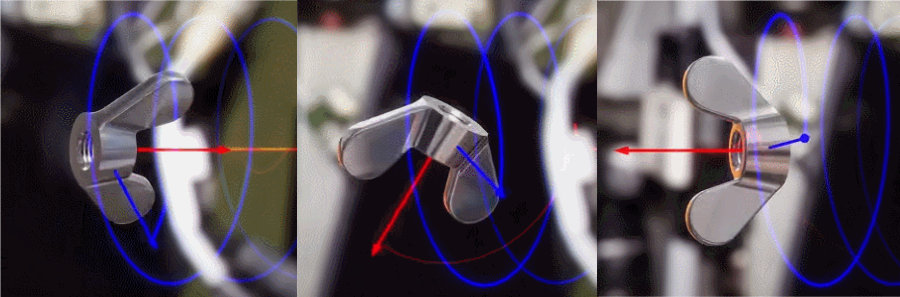
\includegraphics[width=0.9\textwidth]{dzhani.jpg}
\end{center}
   \caption{រូបភាពបង្ហាញអំពីបែបផែន Dzhanibekov \cite{28}។}
\label{fig:10}
\end{figure*}

គោលការណ៍ដែលនៅក្រោយការប្រែប្រួលយ៉ាងឆាប់រហ័សនៃអ័ក្សបង្វិលរបស់ផែនដីគឺស្ថិតនៅលើរូបវិទ្យានៃវត្ថុបង្វិល។ ឧទាហរណ៍ផ្នែកសម្រង់នៃរឿងនេះគឺបែបផែន Dzhanibekov ដែលត្រូវបានស្វែងរកដោយអាស្ត្រូណូតរុស្ស៊ីលោក Vladimir Dzhanibekov \cite{37} ហើយបង្ហាញក្នុងរូបទី \ref{fig:10}។ វត្ថុមួយដែលមិនកំពុងបង្វិលល្អត្រឹមត្រូវលើមួយក្នុងចំណោមអ័ក្សសំខាន់បីនៃសុទ្ធធាតុសង្រ្កាននឹងមិនអាចរក្សាអ័ក្សបង្វិលបង្ហាប់បានទេ។ បើវាបង្វិលជិតអ័ក្សសំខាន់ទីពីរ វានឹងប្រែប្រួលបង្វិលប្រហែលជាឃើញមានការប្រែប្រួលយ៉ាងឆាប់រហ័ស។ ទោះបីជានេះមិនមែនជាអ្វីដែលយើងជឿថាកើតមានក្នុងអំឡុងពេលផែនដីប្រែបង្វិលយ៉ាងឆាប់នោះក៏ដោយ ចំណុចក៏និយាយថាក្រៅករណីសំពាធខាងក្រៅ រូបវិទ្យាបង្វិលប៉ុណ្ណោះដែលអាចពន្យល់អំពីការប្រែប្រួលយ៉ាងឆាប់នៃអ័ក្សបង្វិលផែនដីបាន។

ដើម្បីមានភាពច្បាស់លាស់ ផែនដីប្រហែលជាមិនទទួលបទពិសោធន៍បែបផែន Dzhanibekov ដោយសាមញ្ញនិងស្មើៗគ្នានោះទេ។ បើករណីជាបញ្ហា យើងនឹងអាចរកឃើញអ័ក្សបង្វិលផែនដីប្រែប្រួលបន្តបន្ទាប់ជាយូរយ៉ាងយឺតៗ។ តែជាស្ថានការណ៍ពិត យើងជឿថាផែនដីមានការរំខានរូបវន្តជាប្រចាំ ដោយបណ្តាលឲ្យ "ស្រទាប់ខាងក្រៅបង្វិល" (សែល/ស្រទាប់មេនថល) និង "សារពាង្គកាយបង្វិលខាងក្នុង" (ស្នូល) ត្រូវបានផ្តាច់ចេញពីគ្នា។ មិនមានអាំងពទ័រខាងក្រៅ ទ្រឹស្តីថាមពលបង្វិលថ្នាក់សៀគ្វីនិយាយថា ផែនដីមិនអាចបែរស្រឡះអ័ក្សបង្វិលភ្លាមៗ ទេ ដូច្នេះការផ្តាច់រវាងស្រទាប់ខាងក្រៅនិងស្រទាប់ខាងក្នុងជារឿងមួយប៉ុណ្ណោះក្រៅតែមានសំពាធខាងក្រៅទៅលើផែនដីដែលអាចបណ្តាលឲ្យការបែរយ៉ាងឆាប់និងរ៉ាប់រ៉ៃនេះកើតមាន។

ដំណើរការពិសេសដែលជួយជំរុញឲ្យកើតមានការរំខានខាងក្នុងផែនដីត្រូវគេជឿថាជាការផ្លាស់ប្តូរស្ថានភាពក្នុងរចនាសម្ព័ន្ធធាតុដែកដែលបង្កើតស្នូលផែនដី (រូបទី \ref{fig:11})។ ស្នូលខាងក្នុងរបស់ផែនដីមានសមាសភាពជាថែមដែកបិទខ្ចប់ hcp (hexagonal close-packed Iron (Fe)) \cite{141}។ នៅពេល hcp-Fe ត្រូវបម្លែងទៅជាលើកដែកជាលំនភាពរាវវាបញ្ចេញថាមពលសុិក្ស្យ និងត្រូវបានរុញទៅស្នូលខាងក្រៅ។ ការផ្លាស់ប្តូរស្ថានភាពនេះធ្វើឲ្យទទួលបានសមត្ថភាពអេឡិចត្រូម៉ាញ៉េទិចស្នូលប្រែប្រួល ខ្សោយកម្លាំងម៉ាញ៉េទិចផែនដី និងបញ្ចេញកម្តៅ បង្កើតរចនាសម្ព័ន្ធ LLVP (large low-velocity shear province) (រូបទី \ref{fig:12}) \cite{38} នៅក្នុងស្រទាប់មេនថល និងកម្តៅផ្ទៃផែនដីតាមសមុទ្រច្រពល់។ ទាំងពីររាងផ្សំទាំងនេះត្រូវបានលានតម្លៃយ៉ាងល្អក្នុងសតវត្សថ្មីៗនិងពិភាក្សារក្នុងបត្ថិបក្រោយនៃឯកសារនេះ។

\begin{figure*}[t]
\begin{center}
% \fbox{\rule{0pt}{2in} \rule{.9\linewidth}{0pt}}
\includegraphics[width=1\textwidth]{layers.jpg}
\end{center}
   \caption{ការបង្ហាញពីដំណើរការ​ក្នុងផ្ទៃផែនដី​ដែលនាំឲ្យមានការប្ដូរទិសដៅ ECDO \cite{129}.}
\label{fig:11}
\end{figure*}


\begin{figure}[t]
\begin{center}
% \fbox{\rule{0pt}{2in} \rule{0.9\linewidth}{0pt}}
   \includegraphics[width=1\linewidth]{llvp.jpg}
\end{center}
   \caption{រូបភាពលម្អិតនៃ LLVP នៅក្រោមអាហ្វ្រិកខាងត្បូង \cite{28}.}
\label{fig:12}
\label{fig:onecol}
\end{figure}


ដំណើរការដូចគ្នានេះនៅក្នុងផែនដីដែលកំពុងកើតឡើងវិញជាផ្លូវវិភាគ លោក្សសន្មតថាវាបានជួយជម្រុញឲ្យមានការផ្លាស់ប្តូរទៅស្ថានភាពបង្វិលបច្ចុប្បន្នរបស់ផែនដីវិញក្នុងរយៈពេលខ្លីបន្ទាប់ពីការប្ដូរទិសដៅ។

\section{ភស្ដុតាងសម្រាប់ការប្ដូរទិសដៅផែនដីឆាប់ៗនេះ}
There is strong reason to believe that we are on the brink of another Earth flip. A cataclysm has not occurred for several millennia, which is approximately the frequency with which these events seem to happen based on historical accounts and data. The strongest data supporting an impending flip comes from recent geomagnetic data, which indicates that the Earth's geomagnetic field has been weakening for approximately two thousand years. This weakening has been accelerating and has reached alarming rates in the last few decades.

Depicted in Figure \ref{fig:14} is the geomagnetic field of Earth in 1590 and 2025 \cite{125,126}. As shown in the figure, the field has weakened significantly.

Another metric for the weakening geomagnetic field is the position of the geomagnetic north pole (Figure \ref{fig:13}). Geomagnetic north has historically been located in the Canadian Arctic. However, it has been wandering slowly over the last several centuries, and accelerated significantly a few decades ago. It is now moving rapidly towards Russia at a rate of 55 kilometers per year \cite{124}.

\begin{figure*}[t]
\begin{center}
% \fbox{\rule{0pt}{2in} \rule{.9\linewidth}{0pt}}
\includegraphics[width=0.9\textwidth]{saa.jpg}
\end{center}
   \caption{ការ​បង្ហាញ​ពី​វាល​ឧស្សាហគុណ​ផ្អែក​ពី​ខ្សោយ​ចាប់​ពី​ឆ្នាំ ១៥៩០ ដល់ ២០២៥។ គណនា​ដោយ​ប្រើ​ម៉ូឌែល gufm1 និង IGRF-14 \cite{125,126}។}
\label{fig:14}
\end{figure*}

\begin{figure}[t]
\begin{center}
% \fbox{\rule{0pt}{2in} \rule{1\linewidth}{0pt}}
   \includegraphics[width=1\linewidth]{npw.jpg}
\end{center}
\caption{ទីតាំងប៉ូលខាងជើងម៉ាញេទិចពីឆ្នាំ ១៥៩០ ដល់ ២០២៥ បង្ហាញជាកន្លះ៥ឆ្នាំម្តងៗ \cite{142}.}
\label{fig:13}
\label{fig:onecol}
\end{figure}

\begin{figure}[t]
\begin{center}
% \fbox{\rule{0pt}{2in} \rule{1\linewidth}{0pt}}
   \includegraphics[width=1\linewidth]{ocean-highlight.jpg}
\end{center}
   \caption{អត្រាក្ដៅឡើងរបស់សមុទ្រច្រើនជ្រៅ ($>$2000 ម៉ែត្រ) ពីឆ្នាំ ១៩៩១ ដល់ ២០១០ ប៉ាន់ជុំជាមួយពណ៌ក្រហម \cite{132}.}
\label{fig:15}
\label{fig:onecol}
\end{figure}

វាលម៉ាញេទិចរបស់ភពផែនដីគេជឿថាត្រូវបានបង្កើតដោយដៃណាមូខាងក្នុង - សិលានរង្វង់នៃចរន្តម៉ាឃមាហ្ចមបង្វិលក្នុងស្នូលខាងក្រៅរបស់ផែនដីដោយសារការ​បង្វិលរបស់វា \cite{123}។ ការអន់ខ្សោយនៃវាលម៉ាញេទិចជាលក្ខណៈបង្ហាញថាមានការរំខាននៅជ្រៅក្នុងផែនដី។ យោងទៅតាមទ្រឹស្តី ECDO, ការរំខានទាំងនេះច្រានកំដៅចេញ ហើយចុងក្រោយនាំឱ្យបំបែករវាងស្រទាប់ mantle និងស្នូល បណ្ដាលឱ្យផែនដីត្រឡប់ត្រឡប់ \cite{1}។

មានទិន្នន័យជាច្រើនបញ្ជាក់ពីសកម្មភាពកម្ដៅនៅខាងក្នុងផែនដី។ ភពផែនដីកំពុងក្តៅឡើងត្រូវបានកត់ត្រាក្នុងសីតុណ្ហភាពផ្ទៃដីនិងសមុទ្រឡើងខ្ពស់ \cite{127,128} កម្រិត CO2 ក្នុងបរិយាកាសកើនឡើងស្របទ្រង់ទ្រាយជាមួយចន្លោះកម្ដៅរបស់ផែនដី \cite{129,130} និងការថយចុះនៃផ្ទៃទឹកកកសមុទ្រប្រចាំពិភពលោក \cite{131}។ ទិន្នន័យបង្ហាញថាកម្រិត CO2 និងសីតុណ្ហភាពដែលកើនឡើងមិនមែនជាកត្តាបង្ករ "បណ្ដាលមនុស្សបង្កើត" ប្រើសម្រាប់បម្លែងអាកាសធាតុទេ ទាល់តែរាជធានីនៃតួអនុផលពីស្នូលដែលចេញកំដៅ \cite{129}។

គួរឱ្យសំខាន់បំផុត ការសិក្សាអំពីអត្រាក្ដៅឡើងក្នុងសមុទ្រជ្រៅ ($>$2000 ម៉ែត្រ) បង្ហាញថា មិនត្រឹមតែសមុទ្រជ្រៅកំពុងក្ដៅឡើងទេ ថែមទាំងមានអត្រាក្ដៅឡើងខ្លាំងបំផុតនៅស្រទាប់ abyssal (៤០០០ - ៦០០០ ម៉ែត្រ)។ ក្ដៅសមុទ្រជ្រៅនេះមានមជ្ឈមណ្ឌលនៅក្រោម ៤០០០ ម៉ែត្រ \cite{132,129} ដែលមិនអាចកើតមានបានប្រសិនបើសមុទ្រត្រូវបានកម្ចើតពីលើដោយបរិយាកាស។ ទិន្នន័យបែបនេះបង្ហាញយ៉ាងច្បាស់ថា ការប្រែប្រួលអាកាសធាតុនិងម៉ាញេទិចថ្មីៗនេះត្រូវបានជះឥទ្ធិពលដោយដំណើរការនៅក្រៅក្បាលផែនដី។ រូបភាព \ref{fig:15} បង្ហាញអត្រាឡើងកម្ដៅសមុទ្រ​ជ្រៅពិភពលោកពីឆ្នាំ 1991 ដល់ 2010 \cite{132}។
\section{ការសង់តម្រឹមរបស់ដំណាក់កាលដ៏ជិតមកនៃការប្រែប្រួលផែនទីភពផែនដី}

\begin{figure}[b]
\begin{center}
% \fbox{\rule{0pt}{2in} \rule{1\linewidth}{0pt}}
   \includegraphics[width=1\linewidth]{saa-crop.jpeg}
\end{center}
   \caption{ការគណនាចំណុចបំបែក​មួយបង្កើនលើ Anomaly តំបន់អាត្លង់ទីខាងត្បូង បង្ហាញប្រចាំថ្ងៃទី ១៣ មីនា ឆ្នាំ ២០៥៩ \cite{125,126}។}
\label{fig:16}
\label{fig:onecol}
\end{figure}

ការទស្សនៈពេលវេលានៃការបំបែកបន្តៀតក្រោយបន្ទាប់របស់ផែនដីគឺជាការងារលំបាកមួយ។ បច្ចុប្បន្ន ម៉ូដែលល្អបំផុតដែលយើងមានសម្រាប់នេះ គឺស្ថិតនៅក្នុងទ្រូងដែកម៉ាញេទិចនៃផែនដី - ទម្រង់ភាពអនាមិកអាត្លង់ទីខាងត្បូង (SAA)។ តំបន់នេះលើអាត្លង់ទីខាងត្បូងមានកម្លាំងទ្រូងដែកម៉ាញេទិចខ្សោយបំផុត ហើយត្រូវបានកំណត់ជាតំបន់ដែលមានកម្លាំងទ្រូងដែកម៉ាញេទិចក្រោម ៣២,០០០ នាណូតេសឡា \cite{135} ដែលជាតម្លៃកម្លាំងខ្សោយបំផុតនៅឆ្នាំ ១៥៩០។ ផ្ទៃដី SAA បានកើនឡើងពី ១\% នៃផ្ទៃដីផែនដីនៅឆ្នាំ ១៥៩០ ទៅ ២១\% នៅឆ្នាំ ២០២៥ \cite{136}។

ដើម្បីទទួលយកការព្យាករណ៍ចំពោះពេលដែលផែនដីអាចនឹងបំបែក ខ្ញុំបានបង្ហាញទិន្នន័យផ្ទៃ SAA ជាមួយសមីការចំណុចបំបែក power-law ដែលបង្ហាញអំពីប្រព័ន្ធស្មុគស្មាញមួយដែលជិតមកដល់ផ្លាស់ប្ដូរដ៏សំខាន់មួយ។ ការគណនារបស់ខ្ញុំបានបង្ហាញកាលបរិច្ឆេទចំណុចបំបែកបង្ហាញថាជាថ្ងៃទី ១៣ ខែមីនា ឆ្នាំ ២០៥៩ (រូបភាព \ref{fig:16})។ ការព្យាករណ៍នេះនឹងកាន់តែត្រឹមត្រូវ ខណៈពេលដែលយើងកាន់តែជិតទៅដល់ការផ្លាស់ប្ដូរនោះ \cite{136}។

វិមាត្រផ្សេងទៀតដូចជាការបង្វិលអ័ក្សផែនដី ភាពប្រហែលអាកាសធាតុ និងទិន្នន័យរញ្ជួយដី និងភ្នំភះ ក៏អាចជួយសំរាប់ព្យាករណ៍ពេលដែលការប្រែប្រួលផែនដីបន្ទាប់អាចកើតមានបាន។

\section{ព្រោងកាលបរិច្ឆេទប្រវត្តិសាស្ត្ររបស់ ECDO}
While establishing an exact timeline for past ECDO events is difficult, it seems that there were at least 2 ECDO events during the Holocene. សូមចំណាំអំពីការរាយការណ៍ដែលបានប្រាប់ដោយហេរ៉ូដូតពីព្រះសង្ឃអេហ្ស៊ីបដែលថា \textit{"ចាប់តាំងពីព្រះមហាក្សត្រដំបូងរហូតដល់ព្រះសង្ឃនៃលោកហេផៃស្ទូសដែលបានរាជ្យចុងក្រោយ មានមនុស្សចំនួនប្រាំបីរយនិងសែសិបមួយជំនាន់... ក្នុងពេលនេះពួកគេបាននិយាយថាព្រះអាទិត្យបានផ្លាស់ទីចេញពីទីកន្លែងដើមរបស់ខ្លួនបួនដង ហើយកន្លែងដែលព្រះអាទិត្យលិចឥឡូវនេះ ពួកគេបានឃើញថាខាងនោះព្រះអាទិត្យបានរះពីទីនោះពីរដង ហើយកន្លែងព្រះអាទិត្យរះឥឡូវនេះ ក៏បានឃើញព្រះអាទិត្យលិចពីរដងផងដែរ"} \cite{32}។ ប្លាតុង ដែលរស់នៅក្នុងសតវត្សទីប្រាំមុនគ.ស \cite{111} បាននិយាយថា បន្ទាប់ពីទឹកលិចដ៏ធំមួយដែលលិចក្រុងអាត្លង់ទីសក្នុងមួយថ្ងៃមួយយប់ កាលពី ៩,០០០ ឆ្នាំមុន \textit{"មានទឹកភ្លៀងច្រើនទៀតបានកើតឡើង ហើយអ្នករស់នៅលើភ្នំនោះមិនស្គាល់សិល្បៈនៃការសរសេរទេ ហើយក្នុងបូណ៌ជំនាន់ពួកគេបានផ្តល់ជីវភាពដល់ការរស់នៅ"} \cite{112} ដែលបង្ហាញថាមានការបត់បែនលើសពីពីរដងចាប់តាំងពីបញ្ចប់យង់ហ្គឺដ្រាយ៉ាស ប្រហែលឆ្នាំ ៩៧០០ មុនគ.ស។ ភស្តុតាងផ្លូវរូបវិទ្យាដែលបានររួមទាំងអស់ក្នុងសន្លឹកនេះ និងស្រាវជ្រាវរបស់ខ្ញុំ \cite{2} ផ្ដល់នូវភស្តុតាងច្រើនសម្រាប់បណ្ដាញរបស់ប្លាតុង។

កាលបរិច្ឆេទមួយថ្មីបំផុតសម្រាប់ការបត់បែន ECDO គឺនៅឆមាសចន្លោះឆ្នាំ ២៣០០ ដល់ ១៦០០ មុនគ.ស ដែលគេបានកំណត់ថ្ងៃទៅកាន់របាយការណ៍អំពីទឹកជំនន់ធំៗ (Gun-Yu \cite{113,114,115}, Ogyges \cite{116,117}, ប៉េរូ \cite{118,119}, Exodus \cite{120}) ការបំផ្លាញនៃអធិរាជ្យ និងការបោះបង់ (Mohenjo-Daro \cite{121}, Minoan Crete\cite{100,101}) និងអរិភាពផ្លូវរូបវិទ្យា (bond events \cite{122}, ព្រឹត្តិការណ៍ ៤.២ ពាន់ឆ្នាំ \cite{90})។ គ្មានភស្តុតាងបញ្ចូលគ្នាដ៏ច្រើនដែលថ្មីជាងនេះបង្ហាញពីព្រឹត្តិការណ៍ឧបទ្វិសគ្រោះធំ។

\section{សេចក្តីសន្និដ្ឋាន}

ប្រតិបត្តិការ NANOOK គឺជាការស្ទង់មតិរបស់សហរដ្ឋអាមេរិកក្នុងសម័យសង្គ្រាមត្រជាក់សម្រាប់ផែនទីតំបន់អាគុយ និងឆ្នេរពិភពខាងជើងរបស់សូវៀតបន្ទាប់ពីសង្គ្រាមពិភពលោកលើកទីពីរ \cite{137}។ នៅពេលពួកគេធ្វើការស្រាវជ្រាវ ពួកគេបានរកឃើញថា ខ្សែម៉ាញេទិចស្ថិតនៅជាយឆ្ងាយ 125 ដល់ 200 ម៉ាយ ទៅជើងជាងទីតាំងដែលមែនត្រូវបានបញ្ជាក់ដោយកិច្ចស្រាវជ្រាវពីមុន។ ដូច្នេះ \textit{"ចំពោះអ្នកវិទ្យាសាស្ត្ររដ្ឋាភិបាល បានកើតមានសំណួរមួយថាតើតើអ្វីនឹងកើតឡើងនៅពេលខ្សែម៉ាញេទិច និងខ្សែភូមិសាស្ត្រជួបគ្នា? ដើម្បីឆ្លើយសំណួរនេះ នាយកគម្រោងសាកល្បង ដោយលោក Dr. Paul A. Siple, ស្ថាប័ន RAND Corporation ត្រូវបានជួលអោយស្រាវជ្រាវជាការសាកល្បងនៅក្នុងមណ្ឌល ប្រើម៉ូឌែលផែនដីដែលរួមបញ្ចូលគ្នាដូចជាបាល់បោះផ្សេងៗពីក្នុងទៅក្រៅ — ស្ព៊ឺចុងក្នុងបង្ហាញលក់ដែកដែលមានថ្មប្រើអគ្គីសនីនៃផែនដីដែលខ្សែបញ្ជាក់ “ម៉ាញេទិច” ហើយស្ព៊ឺក្រៅបង្ហាញសំបកផែនដីដែលបង្វិលជុំវិញខ្សែ “ភូមិសាស្ត្រ”។ តាមរយៈការសាកល្បងជាច្រើនលើកបន្តបន្ទាប់គេបានកំណត់ថា នៅពេលខ្សែ “ម៉ាញេទិច” ខិតជិតទៅកាន់ខ្សែ “ភូមិសាស្ត្រ” ខ្សែ “ម៉ាញេទិច” នឹងមានល្បឿនបង្ហាប់កាន់តែខ្លាំងដូចជាត្រូវបានទាញទៅខ្សែ “ភូមិសាស្ត្រ” ដោយកម្លាំងមធ្យមប៉ាន់ និងបានលោតទៅជាប់ខ្សែភូមិសាស្ត្រ; ប៉ុន្តែជំនួសឱ្យខ្សែទាំងពីរជួបគ្នា “ម៉ាញេទិច” នឹង “បត់បែន” ជុំវិញ “ភូមិសាស្ត្រ” ហើយបង្វិលទៅជើងមួយទៀតដូចជាកម្លាំងមេទ្យង់ប៉ាន់នាំឲ្យចេញសេដ្ឋកិច្ចនៅទីតាំងដែលខ្សែទាំងពីរបែកជាយឆ្ងាយប្រហែល ៨៩ ដឺក្រេ។ បន្ទាប់ពីកិច្ចផ្លាស់ប្តូរនេះកើតឡើង ខ្សែទាំងពីរនឹងតុល្យតាំងវិញបន្តិចម្តងៗក្នុងរយៈពេលវែង"} \cite{138,139}។

បន្តបន្ទាប់ \textit{"នៅក្នុងសន្និសីទមួយដែល​សមាជិក Major White បានចូលរួមនៅ Pentagon ដល់ដើមឆ្នាំ ១៩៤៨ អ្នកវិទ្យាសាស្ត្របានពិភាក្សាអំពីភាពសមស្របក្នុងការប្រាប់សាធារណជនអំពីឧប្បកម្មបត់បែនខ្សែពូករបស់ផែនដី។ គ្មានអ្នកវិទ្យាសាស្ត្រណាមួយព្រមរក្សាសម្ងាត់ព័ត៌មាននេះពីសាធារណជនទេ; ប៉ុន្តែម្យ៉ាងទៀតពួកគេក៏មិនអាចព្រមគ្នាផងដែនអំពីរបៀបបង្ហាញព័ត៌មាននេះជាសាធារណៈទេ។ ចំណេះដឹងអំពីរ fenomena នេះ ប្រិយមិត្តមួយចំនួនគិតថា អាចនាំឲ្យសង្គមកន្លះរល៉េកបាន។ ការភ័យខ្លាចរបស់ពួកគេគឺត្រូវបានបង្ហាញថាមិនត្រឹមត្រូវនោះទេ នៅដើមឆ្នាំ ១៩៥០ ព័ត៌មានអំពីវាបានបង្ហោះក្នុងទាំងកាសែតនិងទស្សនាវដ្តីមួយ ប៉ុន្តែមិនបានបង្ករែសព្មភាពតបស្នាមណាមួយពីសាធារណជនដែលសង្កត់ស្ងប់ឬលំបាកជឿ"} \cite{138,139}។

ហេតុអ្វីបានជា​យើងមិនមើលអំពីអ្វីនេះទេ? មានហេតុផលច្រើនគ្រប់គ្រាន់អោយជឿថាភពផែនដីបានបត់បែនមកហើយ។ សន្លឹកនេះរួមទាំងផ្នែកទីពីរនៃអត្ថបទ ផ្ដល់សង្ខេបខ្លីនៃភស្តុតាងពីវិស័យជាច្រើនបង្ហាញថាវាជាករណីដូចដែលទេ​រាយការណ៍ទឹកជំនន់ជុំវិញពិភពលោក ស្រទាប់អំបិលនិងប្រាក់សរសៃសមុទ្រក្រដាសទ្វីប សណ្ដុំក្រោមដីបុរាណ សត្វស្លាប់ និងទេសភាពភូសុខមាតិកាខ្មែង។ មនុស្សត្រូវបានគេ​គិតថាមានអាយុកាលរយៈពេលរយ:កាលច្រើនម៉ឺនឆ្នាំ ប៉ុន្តែប្រវត្តិសាស្ត្រសម័យទំនើបមានត្រឹមប៉ុន្មានពាន់ឆ្នាំតែប៉ុណ្ណោះ។ តើមិនមែនជាករណីថាសពេលណាមួយផែនដីបត់បែន ទ្វីបត្រូវបានខាត់សម្រាំង និងយើងត្រូវតែចាប់ផ្តើមសារជាថ្មីវិញនៅដំណាក់កាលថ្ម ដកនាំអថិថនប្រាសាទសាស្ត្របុរាណរបស់យើងដល់រឿងទុកដាក់ប៉ុណ្ណោះ? ប្រសិនបើបាទដូច្នេះ ការការពារមិនអោយវិបត្តិនេះកើតឡើងម្ដងទៀតក៏អាចជាកិច្ចការសំខាន់បំផុតរបស់មនុស្សជាតិផងដែរ។

ស្របពេលបញ្ចប់ ខ្ញុំនឹងទុកអ្នកជាមួយរឿងរៀងមួយ​ក្នុងសៀវភៅ Timaeus ដែលប្លាតុងបានសរសេរពីការសន្ទនារវាង​សូឡូន មន្រ្តីអាថែន និងបូជាចារ្យអេហ្ស៊ីប \cite{140}: \textit{"ហើយក្នុងឱកាសមួយ ពេលសូឡូនចង់ឲ្យពួកគេសន្ទនាក្នុងប្រវត្តិសាស្ត្រចាស់ៗគេព្យាយាមនិយាយរំពឹងដល់ប្រវត្តិសាស្ត្រចាស់បំផុតរបស់យើង អំពីភូរោនេអុស ដែលប្រាប់ថាជាមនុស្សដំបូង ហើយអំពីនីអូប ហើយគេចាប់ផ្តើមនិយាយរឿងរបស់ Deucalion យ៉ាង Pyrrha បន្ទាប់ពីទឹកជំនន់ ហើយពីរបៀបដែលពួកគេបានរស់ជាប់ក្រោយរាំងដុំទឹកជំនន់ហើយបានប្រាប់ genealogy នៃកូនចៅរបស់ពួកគេ ហើយដោយរាប់ឆ្នាំដល់ព្រឹត្តិការណ៍ក្នុងរឿងរៀងនេះគេចង់ស្វែងរករយះពេលកន្លងទៅ។ នៅពេលនោះបូជាចារ្យម្នាក់ដែលមានអាយុចាស់ជើងមួយបាននិយាយថា សូឡូន សូឡូន អ្នកក្រីកគឺតែងតែជាក្មេង មានតែមនុស្សចាស់មិនមានទេ។ អស់សេចក្តីស្នេហាភាពនេះ គេចាប់ផ្តើមសួរ “ចំពោះទួលម៉េចលើអង្គប្រសាសន៍នេះ?” ខណៈបូជាចារ្យបានឆ្លើយថា “ប្រិយមិត្តអ្នកទាំងអស់គ្នាគឺជាបុគ្គលវ័យក្មេង ព្រោះនៅទីនេះអ្នកមិនបានអានសិល្បៈណាដែលចាស់ៗមកពីសែតែពីប្រវត្តិសាស្ត្រចាស់ៗ អ្នកក៏មិនមានវិទ្យាសាស្ត្រចាស់ក៏ដោយ។ នេះជាមូលហេតុ វានៅតែមានការបំផ្លាញមនុស្សជាច្រើនដំណាក់កាលទៀតដូចជាមានភ្លើងនិងទឹក ជាពិសេសគ្រាន់បន្តិចដោយរបៀបផ្សេងៗ។ ភាសារឿងដែលនិយាយនៅក្នុងប្រទេសអ្នកណ៍ដូចជារឿង Phaethon កូនរបស់ Helios ដែលបានដឹករទេះរបស់ឪពុក ប៉ុន្តែមិនអាចគ្រប់គ្រងបាននោះ រលត់អ្វីៗដែលនៅលើផែនដី ទាំងខ្លួនផ្ទាល់ក៏ស្លាប់ដោយឡើងរាជៈលើផែនដី។ រឿងនេះជារឿងនិទាន ប៉ុន្តេចំពោះមូលហេតុមានទីតាំងផ្លាស់ប្តូរនៃផ្ទៃមេឃនិងការបំផ្លាញដែនដីដោយភ្លើង ជប៉ុនាមួយចំនួន។ នៅពេលនោះអ្នករស់នៅលើភ្នំនិងកន្លែងខ្ពស់នឹងប្រឈមនឹងការបាត់បង់ជាងអ្នកស្ថិតនៅជិតទន្លេឬសមុទ្រ។ ចំពោះរឿងនេះ Nile ដែលជាវិស្សមកាលរបស់យើងបានជួយសង្គ្រោះពួកយើងពីគ្រោះវាសនានេះដោយលើកខ្ពស់។ នៅពេលក្រុមតំណាងមក Gods សម្អាតចេញដោយទឹកភ្លៀង អ្នកលាស់កណ្តាលនឹងបានជួយសង្គ្រោះជាងអ្នកស្ថិតនៅទីក្រុងដែលក្រោមទឹក។ នៅប្រទេសយើង ទឹកមិនធ្លាក់ទេតាមធម្មជាតិវាឡើងរលកពីក្រោម។ ដូច្នេះតំបន់នេះតែងតែជាបុរាណចាស់បំផុត។ មនុស្សនេះតែងតែមានកំណើតកើនចុះ។ ប្រសិនបើមានព្រឹត្តិការណ៍អ្វីត្រូវកើតឡើង ដូចជា Noble បរិសុទ្ធ ឬធំៗ ឬមានឈ្មោះលេចធ្លោ មិនថានៅប្រទេសអ្នក ឬយើង ឬដីផ្សេងទៀតដែលយើងបានស្គាល់និយាយពី ព្រឹត្តិការណ៍ទាំងនេះតែងតែត្រូវបានកត់ត្រាក្នុងប្រាសាទ។ តែក៏អ្នកនិងអ្នកដទៃទៀតតែងតែជាក្រុមថ្មីជានិច្ច។ រាល់ពេលមានរយៈពេលថ្មីទឹកជំនន់មកពួកអ្នកគ្រប់គ្នាត្រូវបានបំបាត់ ចាំតែអ្នកអក្សរ មិនបានយល់ដឹងទេ។ Genealogies ដែលអ្នកបាននិយាយអំពីប្រទេសអ្នកគឺជាកុមារកាន់តែជារឿងនិទាន ដោយសារអ្នកនិយាយតែខ្លះអំពីទឹកជំនន់មួយក្នុងពេលដែលមាននាពេលកន្លងមកជាច្រើនកាន់ស្រាប់។ ជាងនោះទៀតអ្នកមិនដឹងថាជំពូកល្អបំផុតនៃមនុស្សត្រូវបានកើតនៅប្រទេសដែលអ្នករស់នៅនាពេលបច្ចុប្បន្នៗនោះទេ ហើយថានៅលើកំពូលនៃធ្វីបនោះ>> មានមនុស្សមានស្នាមថ្មីដែលសល់ខ្លះៗតែក្មេងៗ ចំពោះវាក៏ត្រូវបានបាត់បង់ជាមួយការបាត់បង់សមត្ថភាពសរសេរ។ មុនពេលមានវាសនាទឹកជំនន់ធំ ព្រះរាជាធានីអាថែនជាការវ័យក្មេងឆ្នើមនិងមានបៀវកម្មល្អឥតខ្ចោះជាងគេ។ គេបាននិយាយថាពួកគេមានសិល្បៈល្អ និងរដ្ឋធម្មនុញ្ញល្អឥតខ្ចោះប្រចាំពិភពលោកដែលយើងបានស្គាល់"}។

បូជាចារ្យដូចគ្នានេះបានប្រាប់សូឡូនអំពីអធិរាជ្យបុរាណកម្មអាត្លង់ទីសផងដែរ៖ \textit{"ក្នុងអ្វីដែលយើងមាននៅទីនេះ ក្រោមមាត់ដែលយើងកំពុងនិយាយនោះជាព្រះបរមបរិជ្ញាម្យ៉ាង ស្រាប់តែមានច្រកចូលតូចមួយ តែពីរោះនេះពិតជាមហាសមុទ្រមួយ ហើយដីនៅជុំវិញវាគួរត្រូវគេហៅថាទ្វីបមួយនៅក្នុងន័យពេញលេញនិងពិតប្រាកដ។ នៅលើកោះអាត្លង់ទីសនេះមានសហភាពព្រះមហាក្សត្រ មានអំណាចធំលើកោះនេះ ជាមួយឣកោះផ្សេងៗទៀត និងជាប់ទៅទ្វីបធំផងដែរ។ ខណៈពេលនេះកងទ័ពទាំងមូលសង្រ្គោះបានប្រមូលផ្តុំគ្នាឡើងចង់ចម្លងទាំងប្រទេសអ្នក និងយើងចូលជាស្អាងមួយ តើគ្មានសង្រ្គោះណាដែលក្លាហានដូចស្ថានភាពប្រទេសរបស់អ្នក។ វាបានការពារឲ្យសេរីភាពចំពោះអ្នកដែលមិនទាន់ឆាប់ដួលចូលក្នុងភាពដួលរលំសង្រ្គោះប្រទេសយើងជាមួយវឌ្ឍនភាពឥតគិតឃើញ។ ប៉ុន្តែពេលក្រោយបានកើតឡើងរញ្ជួយដី និងទឹកជំនន់ធំៗ មួយថ្ងៃមួយយប់ដ៏ក្រួសត្រូវបានហួរកងទ័ពរបស់អ្នកត្រូវបានផ្ទុះជាមួយដី ហើយកោះអាត្លង់ទីសក៏ផុយក្រោមសមុទ្រដែរ"}។

\section{ការសូមអរគុណ}

សូមអរគុណ Ethical Skeptic យើងជាអ្នកនិពន្ធដើមនៃសនិដ្ឋាន ECDO សម្រាប់ការបញ្ចប់បថពិសោធន៍ឆ្លាតវៃរបស់គាត់ និងចែករំលែកនឹងពិភពលោក។ បទនិពន្ធបីជើងរបស់គាត់ \cite{1} ទៅតែស្នាដៃដើមសម្រាប់ទ្រឹស្តី Exothermic Core-Mantle Decoupling Dzhanibekov Oscillation (ECDO) និងមានព័ត៌មានច្រើនជាងដែលខ្ញុំបានលើកឡើងក្នុងនេះ។
Thanks to Ankit, ដែលបានដំណើរការទិន្នន័យប្រមូលផ្ដុំបរិក្ខោសាសន៍នៅតារាង ១ ។

ហើយជាក់ស្តែង អរគុណដល់យក្សដែលពួកយើងឈរនៅលើស្មារបស់ពួកគេ; អ្នកដែលបានធ្វើស្រាវជ្រាវ និងស៊ើបអង្កេតដែលធ្វើឲ្យការងារនេះកើតขึ้นបាន ហើយបានខិតខំបន្ថែមភ្លឺសម្រាប់មនុស្សជាតិ។

\clearpage
\twocolumn

\section{រូបភាពបន្ថែម}

\begin{figure}[H]
\begin{center}
% \fbox{\rule{0pt}{2in} \rule{1\linewidth}{0pt}}
   \includegraphics[width=1\linewidth]{wave.jpg}
\end{center}
   \caption{ការអង្រួនមើលជិតស្ទើរនៅលើការបាក់បែកស៊ុមកោង រលកសឹកកាត់ប៉ារ៉ាបូលីក លើប៉េរ៉ាមីដខាភ្រី \cite{27}។}
\label{fig:19}
\label{fig:onecol}
\end{figure}
\begin{figure}[H]
\begin{center}
% \fbox{\rule{0pt}{2in} \rule{1\linewidth}{0pt}}
   \includegraphics[width=1\linewidth]{star-stone.jpg}
\end{center}
   \caption{ផែនទីផ្កាយដែលបានពីកាត់ចម្លាក់លើថ្មក្នុងមួយច្រកនៃពyramid ខូហ្វូ \cite{28}។}
\label{fig:20}
\label{fig:onecol}
\end{figure}

\begin{figure*}[t]
\begin{center}
% \fbox{\rule{0pt}{2in} \rule{.9\linewidth}{0pt}}
\includegraphics[width=1\textwidth]{deepsea.jpg}
\end{center}
   \caption{រូបភាពនៃភាពខុសគ្នា​របស់ការឡើងកំដៅសមុទ្រជ្រៅ និងជ្រៅបំផុត ប្រៀបធៀប​នឹងខ្សែកោងឡើងកំដៅសមុទ្រធម្មតា។ ភាពខុសគ្នាសរុបនៃការឡើងកំដៅត្រូវបានយកពី NOAA \cite{147} ការចែកចាយកំដៅសមុទ្រជ្រៅ និងជ្រៅបំផុតយកពីសិក្សា​របស់ Desbruyeres \cite{132}, និងដំណើរការទិន្នន័យនិងបង្ហាញដោយ Ethical Skeptic \cite{129}។}
\label{fig:21}
\end{figure*}
\begin{figure*}[t]
\begin{center}
% \fbox{\rule{0pt}{2in} \rule{.9\linewidth}{0pt}}
\includegraphics[width=1\textwidth]{sealevel.jpeg}
\end{center}
   \caption{កម្រិត​ទឹក​សមុទ្រ​បង្ហាញ​កំណើន​ភាពខុសគ្នា ២០\% ជាយូរប្រហែល ៧៥ ឆ្នាំ ជាមួយស្ថានីយ៍ ៦៣ កន្លែង បង្ហាញថាមានកំណើនល្បឿនស្ទឹងទឹក។ ការកើនឡើងនៃភាពខុសគ្នានៃកម្រិតទឹកសមុទ្រជាប់ពេលជាមួយបណ្តាញកម្ដៅសមុទ្រ បង្ហាញថាទាំងពីរនេះអាចបណ្តាលមកពីកម្ដៅពីក្រោមប្រឡាយសមុទ្រនៃផែនដី \cite{2,129}។}
\label{fig:22}
\end{figure*}

\begin{figure*}[t]
\begin{center}
% \fbox{\rule{0pt}{2in} \rule{.9\linewidth}{0pt}}
\includegraphics[width=1\textwidth]{co2.jpg}
\end{center}
   \caption{បរិមាណ CO2 នៅក្នុងបរិយាកាស (ppm) បានកើនឡើងយ៉ាងស្ថិរភាពក្នុងរយៈពេល ៤៥ ឆ្នាំចុងក្រោយនេះ ប្រហែលជាកើតមានដោយសារការកើនឡើងនៃសីតុណ្ហភាពសមុទ្រ។ ប្រភព៖ NOAA \cite{148,129}។}
\label{fig:23}
\end{figure*}

\begin{figure*}[t]
\begin{center}
% \fbox{\rule{0pt}{2in} \rule{.9\linewidth}{0pt}}
\includegraphics[width=1\textwidth]{ice.jpg}
\end{center}
   \caption{ផ្ទៃក្រឡាជាំទឹកកកជាសកល បានកាន់តែតូចចុះក្នុងរយៈពេល៤៥ឆ្នាំចុងក្រោយ ដោយសារដែនដីកំពុងក្ដៅ។ ប្រភព៖ ADS \cite{149}.}
\label{fig:24}
\end{figure*}

\clearpage
\twocolumn

{\small
\renewcommand{\refname}{ឯកសារយោង}
\bibliographystyle{ieee}
\bibliography{egbib}
}

\end{document}